\section{moFitComparator$<$ EOT $>$ Class Template Reference}
\label{classmo_fit_comparator}\index{moFitComparator@{moFitComparator}}
Comparison according to the fitness.  


{\tt \#include $<$moFitComparator.h$>$}

Inheritance diagram for moFitComparator$<$ EOT $>$::\begin{figure}[H]
\begin{center}
\leavevmode
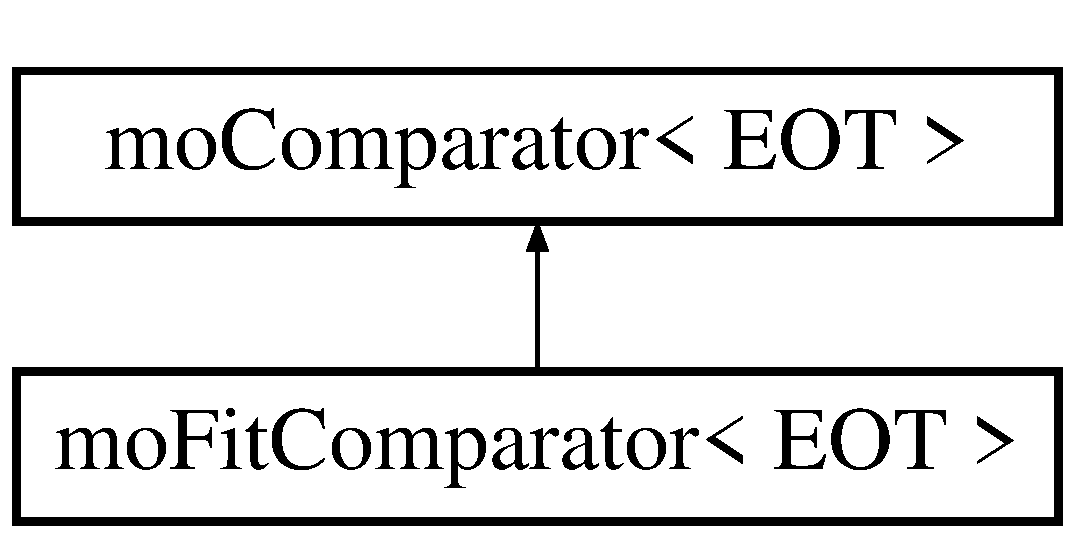
\includegraphics[height=2cm]{classmo_fit_comparator}
\end{center}
\end{figure}
\subsection*{Public Member Functions}
\begin{CompactItemize}
\item 
bool {\bf operator()} (const EOT \&\_\-solution1, const EOT \&\_\-solution2)\label{classmo_fit_comparator_c920d5a49deb16710daf1e5fcde6b16c}

\end{CompactItemize}


\subsection{Detailed Description}
\subsubsection*{template$<$class EOT$>$ class moFitComparator$<$ EOT $>$}

Comparison according to the fitness. 

An EOT is better than an other if its fitness is better. 



Definition at line 20 of file moFitComparator.h.

The documentation for this class was generated from the following file:\begin{CompactItemize}
\item 
moFitComparator.h\end{CompactItemize}
